\section{Evaluation}
\label{sec:evaluation}

%--------------------------------------------------
\begin{figure*}[h!]
  \centering
  
  \begin{subfigure}[b]{0.16\linewidth}
    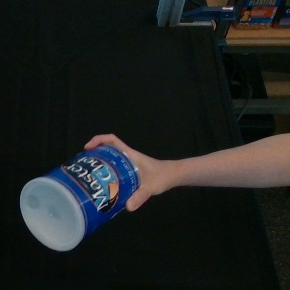
\includegraphics[width=0.98\linewidth]{figs/1000_rgb}
  \end{subfigure}
  \begin{subfigure}[b]{0.16\linewidth}
    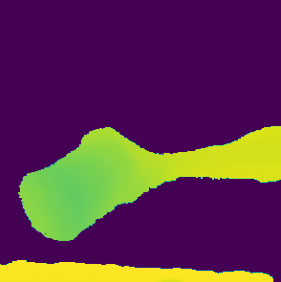
\includegraphics[width=0.98\linewidth]{figs/1000_depth2}
  \end{subfigure}
  \begin{subfigure}[b]{0.16\linewidth}
    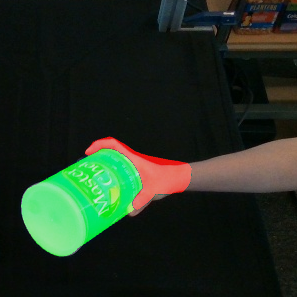
\includegraphics[width=0.98\linewidth]{figs/1000_0}
  \end{subfigure}
  \begin{subfigure}[b]{0.16\linewidth}
    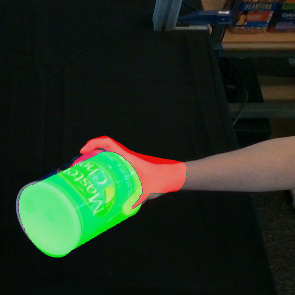
\includegraphics[width=0.98\linewidth]{figs/1000_4}
  \end{subfigure}
    \begin{subfigure}[b]{0.16\linewidth}
    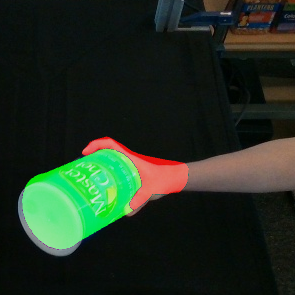
\includegraphics[width=0.98\linewidth]{figs/1000_5}
  \end{subfigure}
    \begin{subfigure}[b]{0.16\linewidth}
    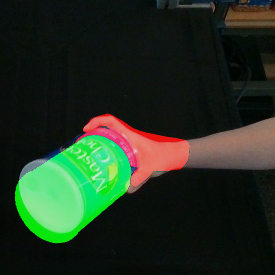
\includegraphics[width=0.98\linewidth]{figs/1000_8}
  \end{subfigure}  
  \vspace{0.2cm}
  
    \begin{subfigure}[b]{0.16\linewidth}
    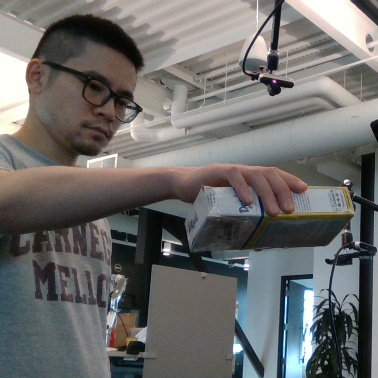
\includegraphics[width=0.98\linewidth]{figs/5319_rgb}
  \end{subfigure}
  \begin{subfigure}[b]{0.16\linewidth}
    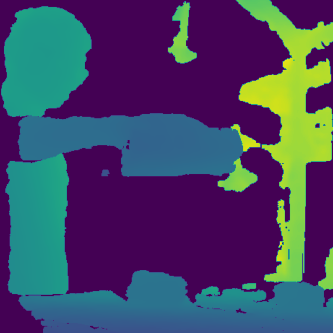
\includegraphics[width=0.98\linewidth]{figs/5319_depth2}
  \end{subfigure}
  \begin{subfigure}[b]{0.16\linewidth}
    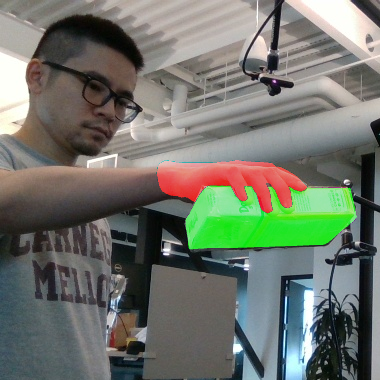
\includegraphics[width=0.98\linewidth]{figs/5319_1}
  \end{subfigure}
  \begin{subfigure}[b]{0.16\linewidth}
    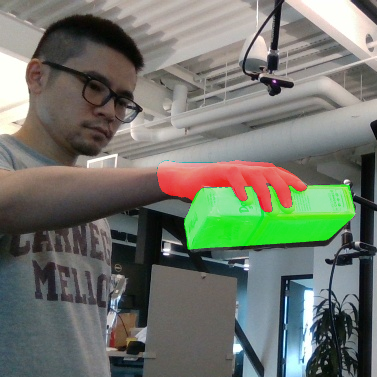
\includegraphics[width=0.98\linewidth]{figs/5319_2}
  \end{subfigure}
    \begin{subfigure}[b]{0.16\linewidth}
    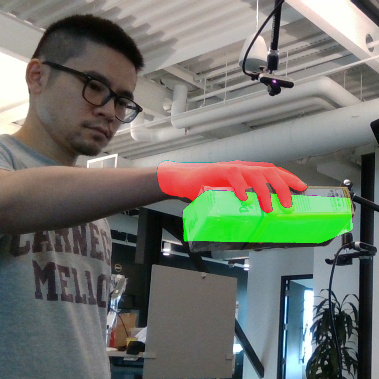
\includegraphics[width=0.98\linewidth]{figs/5319_3}
  \end{subfigure}
    \begin{subfigure}[b]{0.16\linewidth}
    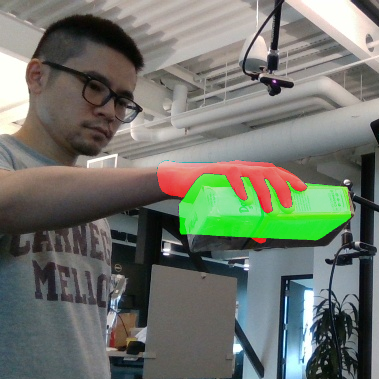
\includegraphics[width=0.98\linewidth]{figs/5319_4}
  \end{subfigure}  
  \vspace{0.2cm}
  
    \begin{subfigure}[b]{0.16\linewidth}
    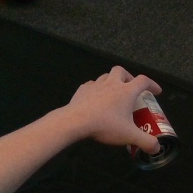
\includegraphics[width=0.98\linewidth]{figs/9063_rgb}
  \end{subfigure}
  \begin{subfigure}[b]{0.16\linewidth}
    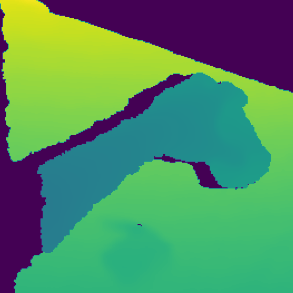
\includegraphics[width=0.98\linewidth]{figs/9063_depth2}
  \end{subfigure}
  \begin{subfigure}[b]{0.16\linewidth}
    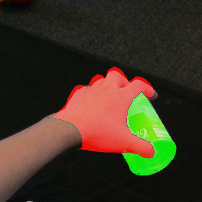
\includegraphics[width=0.98\linewidth]{figs/9063_0}
  \end{subfigure}
  \begin{subfigure}[b]{0.16\linewidth}
    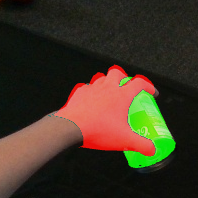
\includegraphics[width=0.98\linewidth]{figs/9063_9}
  \end{subfigure}
    \begin{subfigure}[b]{0.16\linewidth}
    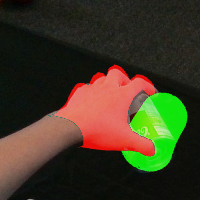
\includegraphics[width=0.98\linewidth]{figs/9063_15}
  \end{subfigure}
    \begin{subfigure}[b]{0.16\linewidth}
    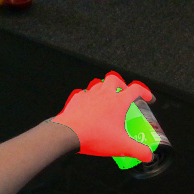
\includegraphics[width=0.98\linewidth]{figs/9063_19}
  \end{subfigure}  
  \vspace{0.2cm}
  
    \begin{subfigure}[b]{0.16\linewidth}
    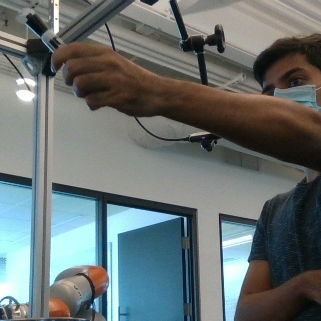
\includegraphics[width=0.98\linewidth]{figs/180000_rgb}
    \caption{RGB}
  \end{subfigure}
  \begin{subfigure}[b]{0.16\linewidth}
    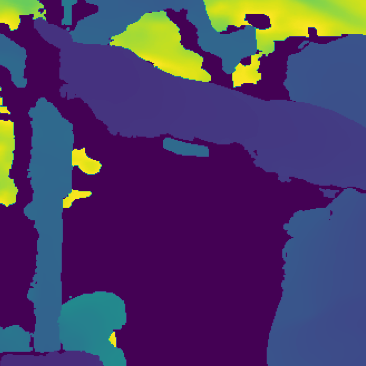
\includegraphics[width=0.98\linewidth]{figs/180000_depth2}
    \caption{Depth}
  \end{subfigure}
  \begin{subfigure}[b]{0.16\linewidth}
    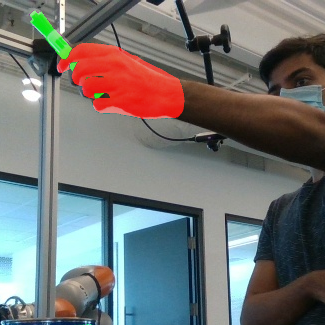
\includegraphics[width=0.98\linewidth]{figs/180000_4}
    \caption{Ground truth}
  \end{subfigure}
  \begin{subfigure}[b]{0.16\linewidth}
    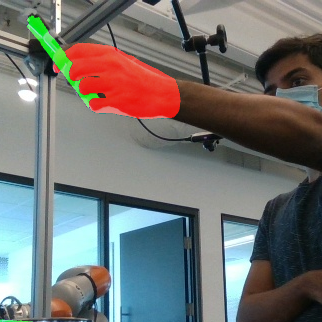
\includegraphics[width=0.98\linewidth]{figs/180000_8}
    \caption{Ours}
  \end{subfigure}
    \begin{subfigure}[b]{0.16\linewidth}
    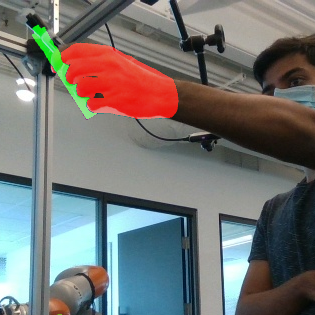
\includegraphics[width=0.98\linewidth]{figs/180000_10}
    \caption{\cite{wang2019densefusion}}
  \end{subfigure}
    \begin{subfigure}[b]{0.16\linewidth}
    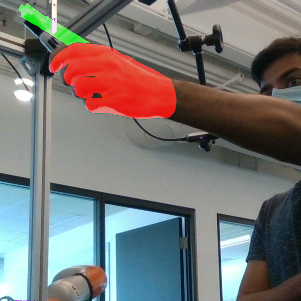
\includegraphics[width=0.98\linewidth]{figs/180000_13}
    \caption{\cite{castro2023crt}}
  \end{subfigure}  
  
  \caption{Qualitative results. (a) and (b) are the input RGBD images. (c) shows the rendered images using ground truth hand and object poses. (d), (e), and (f) display the rendered images using ground truth hand poses and object poses predicted by our method, \cite{wang2019densefusion}, and \cite{castro2023crt}, respectively.}
  \label{fig:result}
\end{figure*}
%--------------------------------------------------

We evaluate our proposed approach on three publicly available datasets: DexYCB (\cite{chao2021dexycb}), FPHAB (\cite{garcia2018first}), and HO-3D (\cite{hampali2020honnotate}). These datasets are chosen for their comprehensive representation of hand-held object interactions, detailed annotations, and diverse scenarios, making them ideal for benchmarking object pose estimation. This evaluation compares our method with state-of-the-art object pose estimation techniques. Furthermore, we assess the impact of our RGB-D fusion module by substituting alternative fusion methods and analyzing the accuracy improvements.

\subsection{Datasets}

\textbf{DexYCB Dataset} (\cite{chao2021dexycb}). This dataset provides 582,000 RGB-D frames across 1,000 sequences with 10 subjects interacting with 20 different objects. Utilizing eight RGB-D cameras, it captures interactions from multiple angles, ensuring rich data diversity. The dataset's precise 3D annotations of both hands and objects make it highly suitable for evaluating hand-held object pose estimation in cluttered environments.

\textbf{FPHAB Dataset} (\cite{garcia2018first}). With over 100,000 frames, this dataset features 45 hand-object interaction categories involving 26 objects. Collected using a motion capture system, it offers detailed 3D annotations, crucial for testing pose estimation models under diverse hand configurations and object manipulations. This diversity aids in assessing the robustness of pose estimation techniques in realistic scenarios.

\textbf{HO-3D Dataset} (\cite{hampali2020honnotate}). Comprising 77,558 frames across 68 sequences, this dataset focuses on challenging hand-object interactions with significant occlusions. It includes RGB images with detailed 3D annotations of hand-object poses, enabling the evaluation of pose estimation methods in complex scenarios. The dataset's challenging conditions test the effectiveness of our approach in real-world applications.

\subsection{\textbf{Implementation Details.}}

All images from each dataset are cropped and resized to $256 \times 256$ pixels. Our implementation\footnote{Our code and other materials are available at \url{https://github.com/papersubm/6d_object_inhand}} uses a pre-trained ResNet34 model, originally trained on ImageNet, as the encoder for RGB images. For point cloud feature extraction, we randomly sample 12,288 points from depth images and use a PointNet++-based feature learning network (\cite{qi2017pointnet++}), which includes 4 set abstraction (SA) layers and 2 feature propagation (FP) layers. Folowing FFB6D (\cite{he2021ffb6d}), we select 256 hand and object keypoints using SIFT-FPS algorithm. The entire system is implemented using PyTorch and Python, running on an NVIDIA RTX-3090 GPU with an Intel Xeon CPU (12 cores, 2.1GHz), utilizing CUDA and the Linux operating system. For all datasets, we use the Adam optimizer with an initial learning rate of 0.01. The learning rate decays by 0.1 at epochs 80, 140, and 200. We train the model with a batch size of 8 and apply standard data augmentation techniques.

\subsection{Evaluation metric}
\label{sec:metric}

To assess the accuracy of the estimated pose $\hat{P}$ relative to the ground-truth pose $\bar{P}$ of an object model $M$, we use the widely adopted Average Distance of Model Points (ADD) metric (\cite{hinterstoisser2012model}). This metric calculates the average distance between corresponding vertices of the object model in the ground-truth pose and the estimated pose. Formally, given the ground truth rotation $\bar{R}$ and translation $\bar{t}$, and the estimated rotation $\hat{R}$ and translation $\hat{t}$, the ADD is defined as:

%----------------------------------------------
\begin{align}
\  ADD = \dfrac{1}{m} \sum_{x \in M} \parallel (\bar{R}x+ \bar{t} - \hat{R}x+ \hat{t}) \parallel
\end{align}
%%%%%%%%%%%%%%%%%%%%%%%%%%%%%%%%%%%%%%%%%%%%%%%%%%%%%%%%%%%%%%%%%%%

\noindent where $m$ is the number of model points. For symmetric objects, we adapt the metric by computing the average distance using the closest point distance method, as in \cite{bregier2017symmetry}. We evaluate the prediction accuracy using average precision ($AP$) (\cite{bregier2017symmetry}). A 6D pose estimate is classified as a true positive if the average distance is less than 10\% of the diameter of the smallest bounding sphere of the object. Additionally, we report the area under the $ADD$ curve ($AUC$) (\cite{wang2019densefusion}), providing a measure of pose estimation performance across varying thresholds.

\subsection{Results}

%-------------------------------------------------
\begin{table}[h]
\caption{Quantitative results on the DexYCB (\cite{chao2021dexycb}), FPHAB (\cite{garcia2018first}), and HO-3D (\cite{hampali2020honnotate}) datasets without Iterative Refinement. Depth-based methods (\cite{wang20216d, gao20206d, guo2021efficient}), RGB methods (\cite{billings2019silhonet, peng2019pvnet, wang2021gdr, castro2023crt}), and RGBD methods (\cite{wang2019densefusion, he2020pvn3d, he2021ffb6d, wu2023geometric, hong2024rdpn6d, lin2024hipose}) are compared with our proposed method (Ours). The runtime for each method is measured in milliseconds (ms).}
\label{tab:dataset_without_ir}
\begin{center}
\begin{tabular}{|l|c|c|c|c|c|c|c|} 
\hline
& \multicolumn{2}{c|}{DexYCB} & \multicolumn{2}{c|}{FPHAB} & \multicolumn{2}{c|}{HO-3D} & Time \\
\hline
Method & $AUC$ & $AP$ & $AUC$ & $AP$ & $AUC$ & $AP$ & $ms$ \\  
\hline 
\cite{wang20216d} & 52.3 & 53.4 & 54.2 & 55.1 & 53.6 & 54.7 & 42 \\
\cite{gao20206d} & 55.4 & 56.1 & 57.3 & 58.2 & 56.7 & 57.6 & 36 \\
\cite{guo2021efficient} & 57.1 & 58.0 & 59.0 & 59.9 & 58.4 & 59.3 & 33 \\
\hline 
\cite{billings2019silhonet} & 54.3 & 55.5 & 56.2 & 57.1 & 55.6 & 56.9 & 35 \\
\cite{peng2019pvnet} & 57.2 & 58.1 & 59.1 & 60.0 & 58.5 & 59.4 & 38 \\
\cite{wang2021gdr} & 59.6 & 60.5 & 61.5 & 62.4 & 60.9 & 61.8 & 32 \\
\cite{castro2023crt} & 61.2 & 62.1 & 63.1 & 64.0 & 62.5 & 63.4 & 30 \\
\hline
\cite{wang2019densefusion} & 60.3 & 61.1 & 62.2 & 63.1 & 61.6 & 62.5 & 42 \\
\cite{he2020pvn3d} & 62.1 & 63.0 & 64.1 & 65.0 & 63.5 & 64.4 & 49 \\
\cite{he2021ffb6d} & 63.4 & 64.2 & 65.3 & 66.2 & 64.8 & 65.7 & 51 \\
\cite{wu2023geometric} & 65.0 & 65.8 & 66.9 & 67.8 & 66.4 & 67.3 & 46 \\
\cite{hong2024rdpn6d} & 66.3 & 67.1 & 68.2 & 69.1 & 67.6 & 68.5 & 55 \\
\cite{lin2024hipose} & 67.5 & 68.4 & 69.6 & 70.5 & 68.9 & 69.8 & 65 \\
Ours & \textbf{80.3} & \textbf{81.2} & \textbf{82.1} & \textbf{83.4} & \textbf{81.5} & \textbf{82.6} & 40 \\
\hline
\end{tabular}
\end{center}
\end{table}
%-------------------------------------------------

\begin{table}[h]
\caption{Quantitative results on the DexYCB (\cite{chao2021dexycb}), FPHAB (\cite{garcia2018first}), and HO-3D (\cite{hampali2020honnotate}) datasets with Iterative Refinement. The runtime for each method is measured in milliseconds (ms).}
\label{tab:dataset_with_ir}
\begin{center}
\begin{tabular}{|l|c|c|c|c|c|c|c|} 
\hline
& \multicolumn{2}{c|}{DexYCB} & \multicolumn{2}{c|}{FPHAB} & \multicolumn{2}{c|}{HO-3D} & Time \\
\hline
Method & $AUC$ & $AP$ & $AUC$ & $AP$ & $AUC$ & $AP$ & $ms$ \\  
\hline 
\cite{wang20216d} & 61.5 & 62.4 & 63.2 & 64.1 & 62.7 & 63.6 & 163 \\
\cite{gao20206d} & 63.2 & 64.0 & 65.1 & 66.0 & 64.5 & 65.3 & 187 \\
\cite{guo2021efficient} & 64.9 & 65.7 & 66.6 & 67.5 & 66.0 & 66.9 & 165 \\
\hline 
\cite{billings2019silhonet} & 62.8 & 63.7 & 64.6 & 65.5 & 63.9 & 64.8 & 160 \\
\cite{peng2019pvnet} & 65.2 & 66.1 & 67.1 & 68.0 & 66.5 & 67.4 & 170 \\
\cite{wang2021gdr} & 66.9 & 67.8 & 68.7 & 69.6 & 68.2 & 69.1 & 185 \\
\cite{castro2023crt} & 68.3 & 69.2 & 70.2 & 71.1 & 69.6 & 70.5 & 178 \\
\hline
\cite{wang2019densefusion} & 67.0 & 67.8 & 68.8 & 69.7 & 68.3 & 69.1 & 240 \\
\cite{he2020pvn3d} & 68.5 & 69.4 & 70.4 & 71.3 & 69.9 & 70.7 & 270 \\
\cite{he2021ffb6d} & 69.8 & 70.7 & 71.7 & 72.6 & 71.2 & 72.0 & 288 \\
\cite{wu2023geometric} & 71.2 & 72.1 & 73.1 & 74.0 & 72.6 & 73.4 & 215 \\
\cite{hong2024rdpn6d} & 72.3 & 73.2 & 74.2 & 75.1 & 73.7 & 74.5 & 265 \\
\cite{lin2024hipose} & 73.5 & 74.4 & 75.4 & 76.3 & 74.9 & 75.7 & 290 \\
Ours & \textbf{86.7} & \textbf{87.2} & \textbf{88.0} & \textbf{88.5} & \textbf{88.3} & \textbf{87.7} & 200 \\
\hline
\end{tabular}
\end{center}
\end{table}

%-------------------------------------------------

Table \ref{tab:dataset_without_ir} and \ref{tab:dataset_with_ir} present the quantitative results, while Figure \ref{fig:result} illustrates the qualitative results. The proposed method achieves the highest accuracy across all datasets in both AUC and AP metrics. For instance, in the DexYCB dataset, our method achieves an AUC of 80.3 and an AP of 81.2 without iterative refinement, and an AUC of 86.7 and an AP of 87.2 with iterative refinement. The results indicate that RGBD-based methods generally outperform RGB-only (\cite{billings2019silhonet, peng2019pvnet, wang2021gdr, castro2023crt}) and depth-only methods (\cite{wang20216d, gao20206d, guo2021efficient}), leveraging the complementary information from both modalities for superior 3D pose estimation. Among the RGBD methods (\cite{wang2019densefusion, he2020pvn3d, he2021ffb6d, wu2023geometric, hong2024rdpn6d, lin2024hipose}), our approach stands out not only for its accuracy but also for its computational efficiency. Despite not being the fastest overall, our method is the fastest among RGBD methods, with a runtime of 40 ms without iterative refinement and 200 ms with iterative refinement, making it feasible for real-world applications. Depth-based methods, such as those by \cite{wang20216d}, \cite{gao20206d}, and \cite{guo2021efficient}, exhibit reasonable speeds but do not achieve the same level of accuracy as RGBD methods. Conversely, RGB methods (\cite{billings2019silhonet, peng2019pvnet, wang2021gdr, castro2023crt}), while faster, sacrifice some accuracy compared to RGBD methods. This balance of high accuracy and competitive speed highlights the practical applicability of our method in real-world scenarios.

%-------------------------------------------------
\begin{table}[h]
\caption{Performance comparison of our method with other state-of-the-art hand-object pose estimation methods. The upper section shows results without iterative refinement, and the lower section includes iterative refinement. The runtime for each method is measured in milliseconds (ms).}
\label{tab:compare_ho}
\begin{center}
\begin{tabular}{|l|c|c|c|c|c|c|c|} 
\hline
& \multicolumn{2}{c|}{DexYCB} & \multicolumn{2}{c|}{FPHAB} & \multicolumn{2}{c|}{HO-3D} & Time \\
\hline
Method & $AUC$ & $AP$ & $AUC$ & $AP$ & $AUC$ & $AP$ & $ms$ \\  
\hline 
\cite{doosti2020hope} & 56.5 & 57.3 & 58.7 & 59.3 & 57.2 & 58.5 & 131 \\
\cite{lin2023harmonious} & 58.7 & 59.5 & 61.8 & 62.1 & 60.0 & 61.1 & 143 \\
\cite{wang2023interacting} & 61.3 & 62.1 & 63.0 & 64.5 & 62.6 & 63.4 & 154 \\
\cite{qi2024hoisdf} & 63.0 & 64.5 & 65.4 & 66.3 & 64.1 & 65.2 & 120 \\
Ours & \textbf{80.3} & \textbf{81.2} & \textbf{82.1} & \textbf{83.4} & \textbf{81.5} & \textbf{82.6} & 40 \\
\hline
\cite{doosti2020hope} & 65.2 & 67.1 & 66.2 & 67.0 & 64.3 & 67.0 & 461 \\
\cite{lin2023harmonious} & 69.0 & 71.2 & 69.0 & 70.7 & 68.1 & 69.0 & 496 \\
\cite{wang2023interacting} & 69.3 & 70.4 & 71.2 & 73.8 & 70.1 & 71.8 & 535 \\
\cite{qi2024hoisdf} & 70.7 & 72.6 & 73.0 & 75.3 & 72.4 & 74.2 & 422 \\
Ours & \textbf{86.7} & \textbf{87.2} & \textbf{88.0} & \textbf{88.5} & \textbf{88.3} & \textbf{87.7} & 200 \\
\hline
\end{tabular}
\end{center}
\end{table}
%-------------------------------------------------

We further compare the proposed method with joint hand-object pose estimation approaches, as shown in Table~\ref{tab:compare_ho}. It is important to note that we evaluate the performance exclusively on object pose estimation, even though the compared methods estimate both hand and object poses. By focusing solely on object pose estimation, our method avoids the complexities inherent in modeling hand articulations. The model is simpler, with fewer parameters, making it easier to train and less prone to overfitting. This design choice results in a more streamlined and accurate estimation process, leading to significantly higher AUC and AP scores across all datasets. For instance, without iterative refinement, our method achieves an AUC of 80.3 and an AP of 81.2 on the DexYCB dataset, compared to 63.0 and 64.5, respectively, for the method by \cite{qi2024hoisdf}. On the FPHAB dataset, our method obtains an AUC of 82.1 and an AP of 83.4, far outperforming \cite{qi2024hoisdf}, which achieves 65.4 and 66.3. The same trend continues on the HO-3D dataset, where our method achieves an AUC of 81.5 and an AP of 82.6, compared to 64.1 and 65.2 for \cite{qi2024hoisdf}. Moreover, the exclusion of hand pose estimation not only enhances accuracy but also significantly improves runtime efficiency. Our method operates at 40 ms without iterative refinement and 200 ms with iterative refinement, which is considerably faster than joint estimation methods such as \cite{lin2023harmonious}, which requires 143 ms and 496 ms. These results clearly demonstrate the advantages of simplifying the problem to focus exclusively on object pose estimation, particularly in applications where the object's pose is more critical than the hand's, such as inventory scanning and mobile AR. By concentrating on this primary task, we achieve both higher accuracy and faster performance, validating our approach as a practical and effective solution for hand-held object pose estimation in complex, occluded environments.


\subsection{Ablation Study}

%-------------------------------------------------
\begin{table}[h]
\caption{Ablation study without Iterative Refinement. The table compares our full method with versions that exclude hand keypoint voting (w/o hand keypoints), the vote-based fusion module using channel attention (w/o $\mathcal{M}_{fus}$), and hand-aware object pose estimation using self-attention (w/o $\mathcal{M}_{hao}$).}
\label{tab:ablation_without_ir}
\begin{center}
\begin{tabular}{|l|c|c|c|c|c|c|c|} 
\hline
& \multicolumn{2}{c|}{DexYCB} & \multicolumn{2}{c|}{FPHAB} & \multicolumn{2}{c|}{HO-3D} & Time \\
\hline
Method & $AUC$ & $AP$ & $AUC$ & $AP$ & $AUC$ & $AP$ & $ms$ \\  
\hline 
w/o hand keypoints & 76.2 & 77.1 & 76.8 & 79.3 & 75.2 & 77.6 & 38 \\

w/o $\mathcal{M}_{fus}$ & 70.5 & 71.3 & 71.4 & 72.1 & 68.4 & 70.2 & 39 \\

w/o $\mathcal{M}_{hao}$ & 77.8 & 79.2 & 77.5 & 79.7 & 76.3 & 77.8 & 40 \\

Full & \textbf{80.3} & \textbf{81.2} & \textbf{82.1} & \textbf{83.4} & \textbf{81.5} & \textbf{82.6} & 40 \\
\hline
\end{tabular}
\end{center}
\end{table}
%-------------------------------------------------

\begin{table}[h]
\caption{Ablation study with Iterative Refinement.}
\label{tab:ablation_with_ir}
\begin{center}
\begin{tabular}{|l|c|c|c|c|c|c|c|} 
\hline
& \multicolumn{2}{c|}{DexYCB} & \multicolumn{2}{c|}{FPHAB} & \multicolumn{2}{c|}{HO-3D} & Time \\
\hline
Method & $AUC$ & $AP$ & $AUC$ & $AP$ & $AUC$ & $AP$ & $ms$ \\  
\hline 
w/o hand keypoints & 84.2 & 85.1 & 86.1 & 86.5 & 85.2 & 85.0 & 190 \\

w/o $\mathcal{M}_{fus}$ & 75.5 & 75.6 & 76.3 & 76.8 & 75.4 & 75.7 & 268 \\

w/o $\mathcal{M}_{hao}$ & 84.5 & 85.6 & 85.6 & 86.3 & 85.8 & 85.3 & 192 \\

Full & \textbf{86.7} & \textbf{87.2} & \textbf{88.0} & \textbf{88.5} & \textbf{88.3} & \textbf{87.7} & 200 \\
\hline
\end{tabular}
\end{center}
\end{table}
%-------------------------------------------------

The ablation study reveals the significance of each component in our method for RGBD fusion in hand-held object pose estimation (see Table \ref{tab:ablation_without_ir} and \ref{tab:ablation_with_ir}). Removing the hand keypoint voting mechanism resulted in a notable drop in performance across all datasets and metrics. For instance, without hand keypoints, the AUC decreased from 80.3 to 76.2 on DexYCB, 82.1 to 76.8 on FPHAB, and 81.5 to 75.2 on HO-3D. This highlights the critical role of hand keypoint voting in enhancing the accuracy of pose estimation by providing valuable spatial cues. The exclusion of the vote-based fusion module using channel attention ($\mathcal{M}_{fus}$) led to the most significant performance drop, with the AUC falling to 70.5, 71.4, and 68.4 on DexYCB, FPHAB, and HO-3D, respectively. This substantial decrease underscores the importance of the vote-based fusion module in effectively combining RGB and depth features, which is crucial for accurate pose predictions. Removing the hand-aware object pose estimation module ($\mathcal{M}_{hao}$) caused a moderate decrease in performance. The AUC dropped to 77.8, 77.5, and 76.3 on DexYCB, FPHAB, and HO-3D, respectively. The self-attention mechanism that learns the relationship between the hand and the object significantly contributes to the overall accuracy of pose estimation, even though it is not as critical as the vote-based fusion module. The full model, incorporating all components, achieved the highest performance across all datasets and metrics, with an AUC of 80.3, 82.1, and 81.5 on DexYCB, FPHAB, and HO-3D, respectively. This confirms the effectiveness of our proposed method and the synergistic benefits of combining hand keypoint voting, vote-based fusion with channel attention, and hand-aware object pose estimation. The computational time for the full model is 40 ms without iterative refinement and 200 ms with iterative refinement, which, despite a slight increase compared to some ablated versions, remains within a reasonable range. These results justify the additional computational cost, making the full model the most robust and accurate for hand-held object pose estimation.

\section{Conclusion}

In this paper, we have introduced a novel deep neural network designed for the 6D pose estimation of hand-held objects using RGB-D images. Our approach tackles the significant challenges posed by occlusions from the hand and the complexities in effectively fusing RGB and depth data.  Our network leverages a voting scheme where both 2D and 3D keypoints cast votes for the object's pose, significantly enhancing the estimation in scenarios with occluded objects. Additionally, we model the interaction between the hand and the object through a self-attention mechanism, which captures complex spatial relationships and improves the robustness of the pose estimation process. Extensive experiments on three public datasets demonstrate that our method outperforms existing approaches in terms of accuracy and robustness. Our vote-based RGBD fusion framework offers a promising solution for hand-held object pose estimation, particularly in challenging scenarios involving occlusions and complex hand-object interactions. Future work will focus on further improving the efficiency of the model and exploring its application to a broader range of objects and environments. \\